\documentclass{beamer}
\usepackage{amsmath, bm}
%
% Choose how your presentation looks.
%
% For more themes, color themes and font themes, see:
% http://deic.uab.es/~iblanes/beamer_gallery/index_by_theme.html
%
\mode<presentation>
{
  \usetheme{Madrid}      % or try Darmstadt, Madrid, Warsaw, ...
  \usecolortheme{beaver} % or try albatross, beaver, crane, ...
  \usefonttheme{serif}  % or try serif, structurebold, ...
  \setbeamertemplate{navigation symbols}{}
  \setbeamertemplate{caption}[numbered]
} 

\setbeamertemplate{caption}{\raggedright\insertcaption\par}

\usepackage[english]{babel}
\usepackage[utf8]{inputenc}
\usepackage[T1]{fontenc}
\usepackage{graphicx}
\usepackage{tikz}
\usetikzlibrary{shapes,snakes,arrows, chains, positioning, shapes.geometric, shapes.symbols,calc,shadows}



%tikzxommand
\def\centerarc[#1](#2)(#3:#4:#5)% Syntax: [draw options] (center) (initial angle:final angle:radius)
{ \draw[#1] ($(#2)+({#5*cos(#3)},{#5*sin(#3)})$) arc (#3:#4:#5); }


%commands
\newcommand{\C}{\mathbb{C}}
\newcommand{\R}{\mathbb{R}}
\newcommand{\CP}{\mathbb{CP}}
\newcommand{\mM}{\mathcal{M}}
\newcommand{\mL}{\mathcal{L}}

\newcommand{\mH}{\mathcal{H}}

\newcommand{\ddb}{\partial\overline{\partial}}
\DeclareMathOperator{\Met}{Met}
\DeclareMathOperator{\codim}{codim}
\DeclareMathOperator{\mul}{mult}
\DeclareMathOperator{\hot}{(h.o.t.)}

\newcommand{\mathcolorbox}[2]{\colorbox{#1}{$\displaystyle #2$}}

\title[]{A Miyaoka-Yau inequality for hyperplane arrangements in \(\CP^d\)}
\author[Martin de Borbon]{Martin de Borbon (joint with Dmitri Panov)}
\institute[Loughborough]{Living on the edge of the moduli space, Aarhus}
\date[18 May, Aarhus]{18-22 May 2026}

\begin{document}


\begin{frame}
  \titlepage
\end{frame}

\section{Outline}
\begin{frame}
	\frametitle{Outline}
	\begin{itemize}
		\setlength{\itemsep}{\fill}
		
		\pause
		\item Introduction: 
		constant curvature metrics on Riemann surfaces with conical singularities
		
		\pause
		\item Main result: 
		polyhedral K\"ahler metrics on \(\CP^d\)
		
		\pause
		\item Sketch proof: 
		Kobayashi-Hitchin correspondence for parabolic bundles  
		
		\pause
		\item Conjectures: 
		K\"ahler-Einstein metrics and Miyaoka-Yau inequality for log pairs
	\end{itemize}
\end{frame}

\section{Riemann surfaces}

\begin{frame}
	\frametitle{Metrics on surfaces with conical singularities}
	\pause
	Let \(\Sigma\) be a compact orientable 2D surface.
	\pause
	Let \(p_1, \ldots, p_n \in \Sigma\) and let \(\alpha_1, \ldots, \alpha_n >0\).
	\pause
	Let \(g\) be a metric on \(\Sigma \setminus \{p_1, \ldots, p_n\}\) with constant curvature \(K = 1, 0, -1\) that near \(p_i\) is locally isometric to
	\[
	\begin{cases}
	dr^2 + \alpha_i^2 \sin^2(r) d\theta^2 \\
	dr^2 + \alpha_i^2 r^2 d\theta^2 \\
	dr^2 + \alpha_i^2 \sinh^2(r) d\theta^2 
	\end{cases}
	\]
	\pause
	Examples: double of a polygon;
	\pause 
	surface of a polyhedron.
	\pause
	\textbf{Gauss-Bonnet}
	\[
	\frac{1}{2\pi} \int_{\Sigma} K dA = \chi(\Sigma) + \sum_{i=1}^{n} (\alpha_i-1)
	\]
	\pause
	Metric + orientation \(\implies\) Riemann surface \(X\) 
\end{frame}

\begin{frame}
	\frametitle{McOwen (1988), Troyanov (1991)}
	\pause
	Let \(X\) be a compact Riemann surface. 
	\pause
	Let \(x_1, \ldots, x_n \in X\) and let \(\bm{\alpha} = (\alpha_1, \ldots, \alpha_n) \in (\R_{>0})^n\). 
	\pause
	Define
	\[
	\chi(X, \bm{\alpha}) = \chi(X) + \sum_{i=1}^{n} (\alpha_i - 1)
	\]
	\begin{itemize}
		\pause
		\item If \(\chi(X, \bm{\alpha}) < 0\) then there exists a unique  K\"ahler metric on \(X\) with \(K_g = -1\) and cone angle \(2\pi\alpha_i\) at \(x_i\)
		\pause
		\item If \(\chi(X, \bm{\alpha}) =0\) then there exists a unique up to scale  K\"ahler metric on \(X\) with \(K_g = 0\) and cone angle \(2\pi\alpha_i\) at \(x_i\)
		\pause
		\item If \(\chi(X, \bm{\alpha}) > 0\). 
		\pause
		Furthermore, assume that \(\alpha_i \in (0,1)\) and \(n \geq 3\).
		\pause
		Then there exists a unique  K\"ahler metric on \(X = \CP^1\) with \(K_g = 1\) and cone angle \(2\pi\alpha_i\) at \(x_i\) if and only if
		\[
		\forall i \quad
		a_i < \frac{1}{2} \cdot \sum_{i=1}^{n} a_i  \quad \textup{ where } a_i = 1-\alpha_i
		\]
	\end{itemize}
\end{frame}


\section{Main result}
\begin{frame}
	\frametitle{Main result}
	\pause
	\begin{theorem}[Panov 2009 when \(d=2\), dB-Panov 2025-26 for \(d \geq 2\)]
		Let \(\mH = \{H_1, \ldots, H_n\}\) be a hyperplane arrangement in \(\CP^d\) with \(d \geq 1\). 
		\pause
		Let \(\alpha_1, \ldots, \alpha_n \in (0,1)\). Write \(a_i = 1-\alpha_i\). 
		\pause
		Assume that:
		\begin{enumerate}
			\pause
			\item\label{it:cy} \(\sum_{i=1}^{n} a_i = d+1\)
			\pause
			\item the weighted arrangement \(\{(H_i,a_i)\}_{i=1}^n\) is \textbf{stable}
		\end{enumerate}
		\pause
		Then the following inequality holds:
		\begin{equation}\label{eq:my}
		Q(a_1, \ldots, a_n) \leq 0 	
		\end{equation}
		where \(Q\) is the \textbf{Hirzebruch quadratic form} of \(\mH\). 
		\pause
		Moreover, the equality holds if and only if there exists a \textbf{polyhedral K\"ahler \textup{(PK)}} metric on \(\CP^d\) with cone angles \(2\pi\alpha_i\) along \(H_i\).
	\end{theorem}
\end{frame}


\begin{frame}
	\frametitle{Hirzebruch (1983-85)}
	\begin{center}
		\begin{figure}
			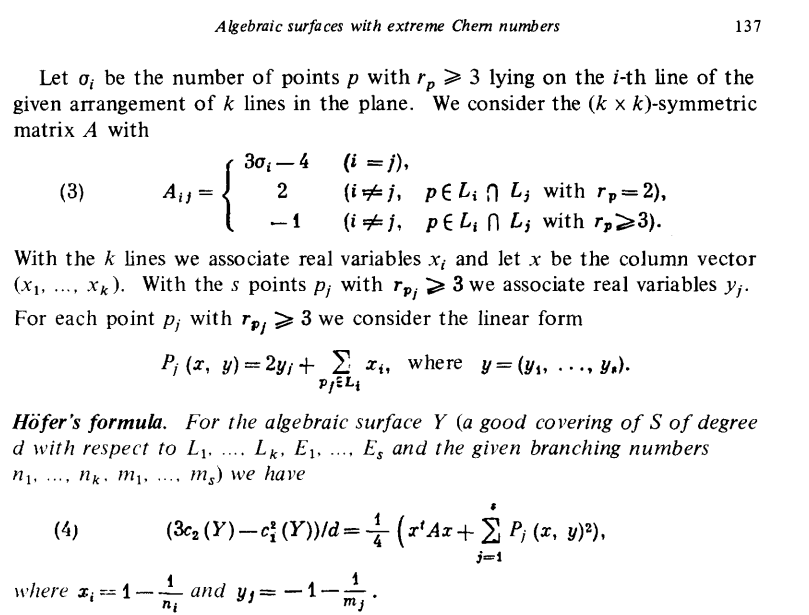
\includegraphics[width=0.8\textwidth,height=0.8\textheight,keepaspectratio]{hofer}
		\end{figure}
	\end{center}
\end{frame}

\section{proof}
\begin{frame}
	\frametitle{Sketch proof}
	Follow Panov (2009) 
	\begin{itemize}
		\pause
		\item Take a log resolution \(\pi: X \to \CP^d\)
		\pause
		\item Define a parabolic structure \(E_*\) on \(E = \pi^*T\CP^d\)
		\begin{enumerate}
			\pause
			\item \(\mathrm{parc}_1(E_*) = 0 \iff \sum_{i=1}^{n} a_i = d+1\)
			\pause
			\item \(E_*\) is slope stable \(\iff\) \(\{(H_i,a_i)\}_{i=1}^n\) is stable
			\pause
			\item \(\mathrm{parch}_2(E_*) = 0 \iff Q(a_1, \ldots, a_n) = 0\)
		\end{enumerate}
		\pause
		\item Apply the Kobayashi-Hitchin correspondence for parabolic bundles (Mochizuki, 2006) to obtain a \emph{flat unitary logarithmic connection} \(\widetilde{\nabla}\) on \(E\) adapted to the parabolic structure
		\pause
		\item \(\widetilde{\nabla} = \pi^*\nabla\) where \(\nabla\) is a torsion-free (flat, unitary, logarithmic) connection on \(T\CP^n\)
		\pause
		\item \(\nabla\) is the Levi-Civita connection of a flat K\"ahler metric \(g\) on the arrangement complement whose metric completion is polyhedral 
	\end{itemize}
\end{frame}

\section{conjectures}
\begin{frame}
	\frametitle{Questions}
	\begin{itemize}
		\pause
		\item Which arrangements admit PK metrics?
		\pause
		\item Suppose \((X, \Delta)\) is a klt pair endowed with a weak KE metric \(g\)
		\begin{enumerate}
			\pause
			\item When does \(g\) have constant holomorphic sectional curvature?
			\pause
			\item Is \(|\mathrm{Riem}(g)|^2\) locally integrable near the conical divisor?
			\pause
			\item If \(g\) is flat, does it need to be polyhedral?
		\end{enumerate}
	\pause
	\item Are there any other examples of PK manifolds with cone angles less than \(2\pi\) besides complex projective space and products?
	\end{itemize}
\pause
\begin{center}
	\Huge{THANK YOU!}
\end{center}
\end{frame}





\end{document}
